\chapter{Results and discussions}
\label{chp:resdisc}

\section{HLS output from LegUp}
As a quick introduction to how the output from LegUp looks, we will have a look at a simple example and what the output looks like. Since the code output is very large, it will be of more use to look at a figure describing the different parts of the code and how it is connected. Beware that this section describes output from LegUp when it is freshly installed, without any alterations or changes so setting. In general, the modules declared in the output Verilog file are these:
\begin{compactdesc}
    \item[top]Top module for Verilog. Instantiates main and memory\_controller modules.
    \item[main]Main function from C project. Contains \gls{fsm} that handles all functionality from original C program.
    \item[memory\_controller]Contains global memories and logic for reading and writing to memory. Instantiates as many ram\_dual\_port and rom\_dual\_port modules as necessary.
    \item[ram\_dual\_port] Dual port RAM module used inside memory controller for global memories.
    \item[rom\_dual\_port] Dual port ROM module used inside memory controller for global memories.
    \item[\%board\%]FPGA specific top module. Instantiates top-module and 8 hex{\textunderscore}digits modules and connects return\_value from top to hex modules for visualizing the results.
    \item[circuit\_start\_control]FPGA specific module. 
    \item[hex\_digits]FPGA specific module. Controls hex LEDs for visualization of results.
    \item[main\_tb]Basic testbench that can be used for simulation. Instantiates top-module. Testbench code generates \textit{clk} signal and applies \textit{reset} and \textit{start} signals to the module before waiting for finish flag. There are no additional input stimuli, so this needs to be added manually by the user.
\end{compactdesc}

\noindent
Listing \ref{lst:exampleCProgram} shows a simple C implementation of a square-root approximation. The reason that the arguments to the main function are given in this way, is described in \cref{subsec:inoutprobs}. \gls{hls} is performed by running \verb!make!. The output Verilog file contains over 3000 lines of code and can therefore not be presented her, it would anyway not give much information.
\begin{lstlisting}[caption={Useless code},label=lst:exampleCProgram]
#define abs(a) ( ((a) < 0) ? -(a) : (a) )
#define max( a, b ) ( ((a) > (b)) ? (a) : (b) )
#define min( a, b ) ( ((a) < (b)) ? (a) : (b) )

// square-root approximation:
int main(int inDataA, char *inDataB[]) {

    int x = max(abs(inDataA), abs(*inDataB[0]));
    int y = min(abs(inDataA), abs(*inDataB[0]));

    return max(x, x-(x>>3)+(y>>1));
}
\end{lstlisting}
\noindent
A project in Quartus can be created by running \verb!make p! and a full compilation can be executed by running \verb!make f!. The top module netlist of the example from \cref{lst:exampleCProgram} can be seen in \cref{fig:legupouttop}
\begin{figure}[hbpt]
\centering
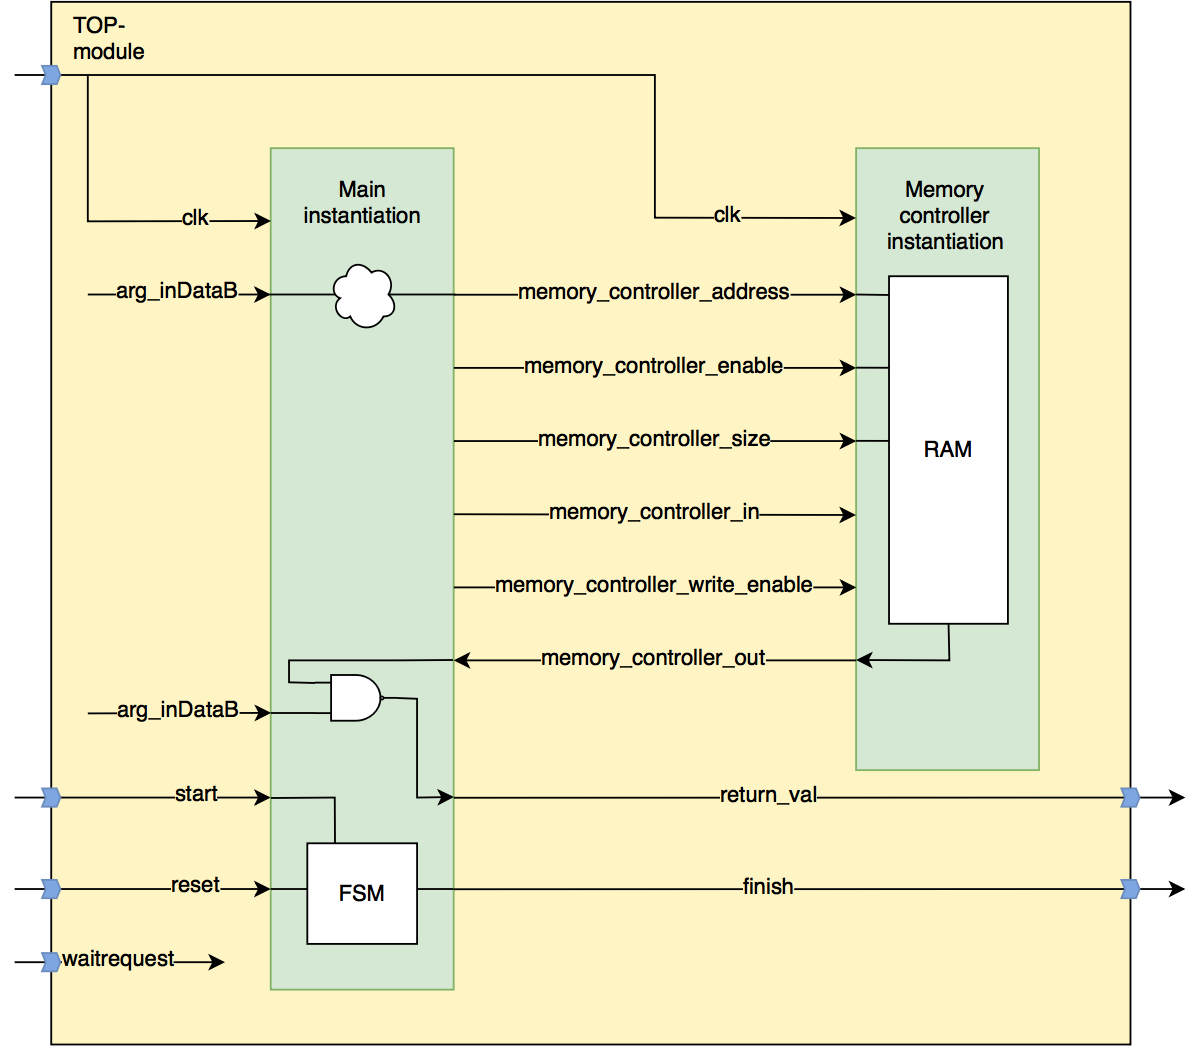
\includegraphics[width=0.8\textwidth]{../figs/LegUpOutputTop.png}
\caption{\label{fig:legupouttop}Top module of HLS-generated Verilog from LegUp synthesized in Quartus}
\end{figure}
Notice that the inputs to the instantiated main module, inDataA and inData,B does not propagate to the top module instantiation. Also, if we look inside the main module, shown in \cref{fig:legupoumain}, inDataB is only mapped to the signal \textit{memory\_controller\_address\_a}. This is because inDataB is decleared as a pointer in the C code, meaning that the input only provides the address to a location in memory where the data can be fetched. This issue is discussed further in \cref{sec:encprob}.

\begin{figure}[hbpt]
\centering
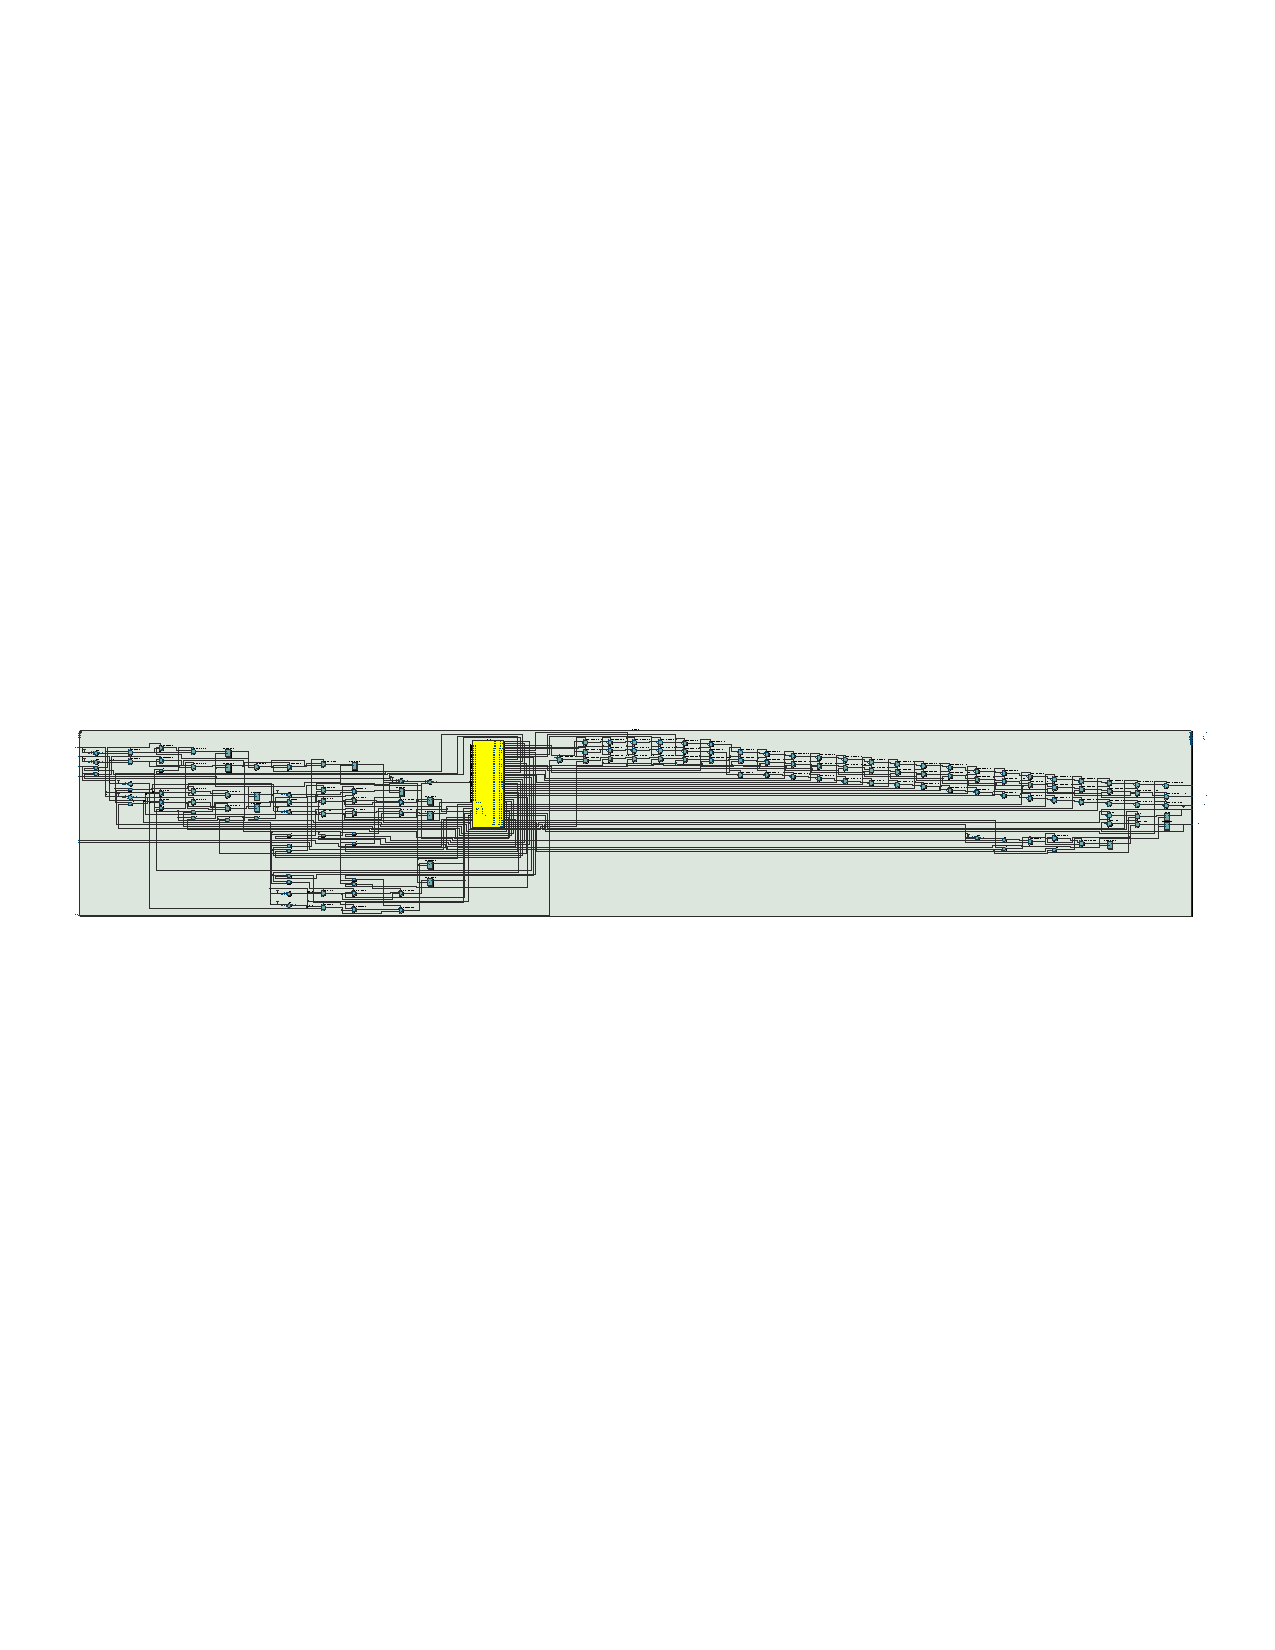
\includegraphics[trim=1cm 12cm 1cm 12cm,clip=true, width=\textwidth]{../figs/LegUpOutputMain.pdf}
%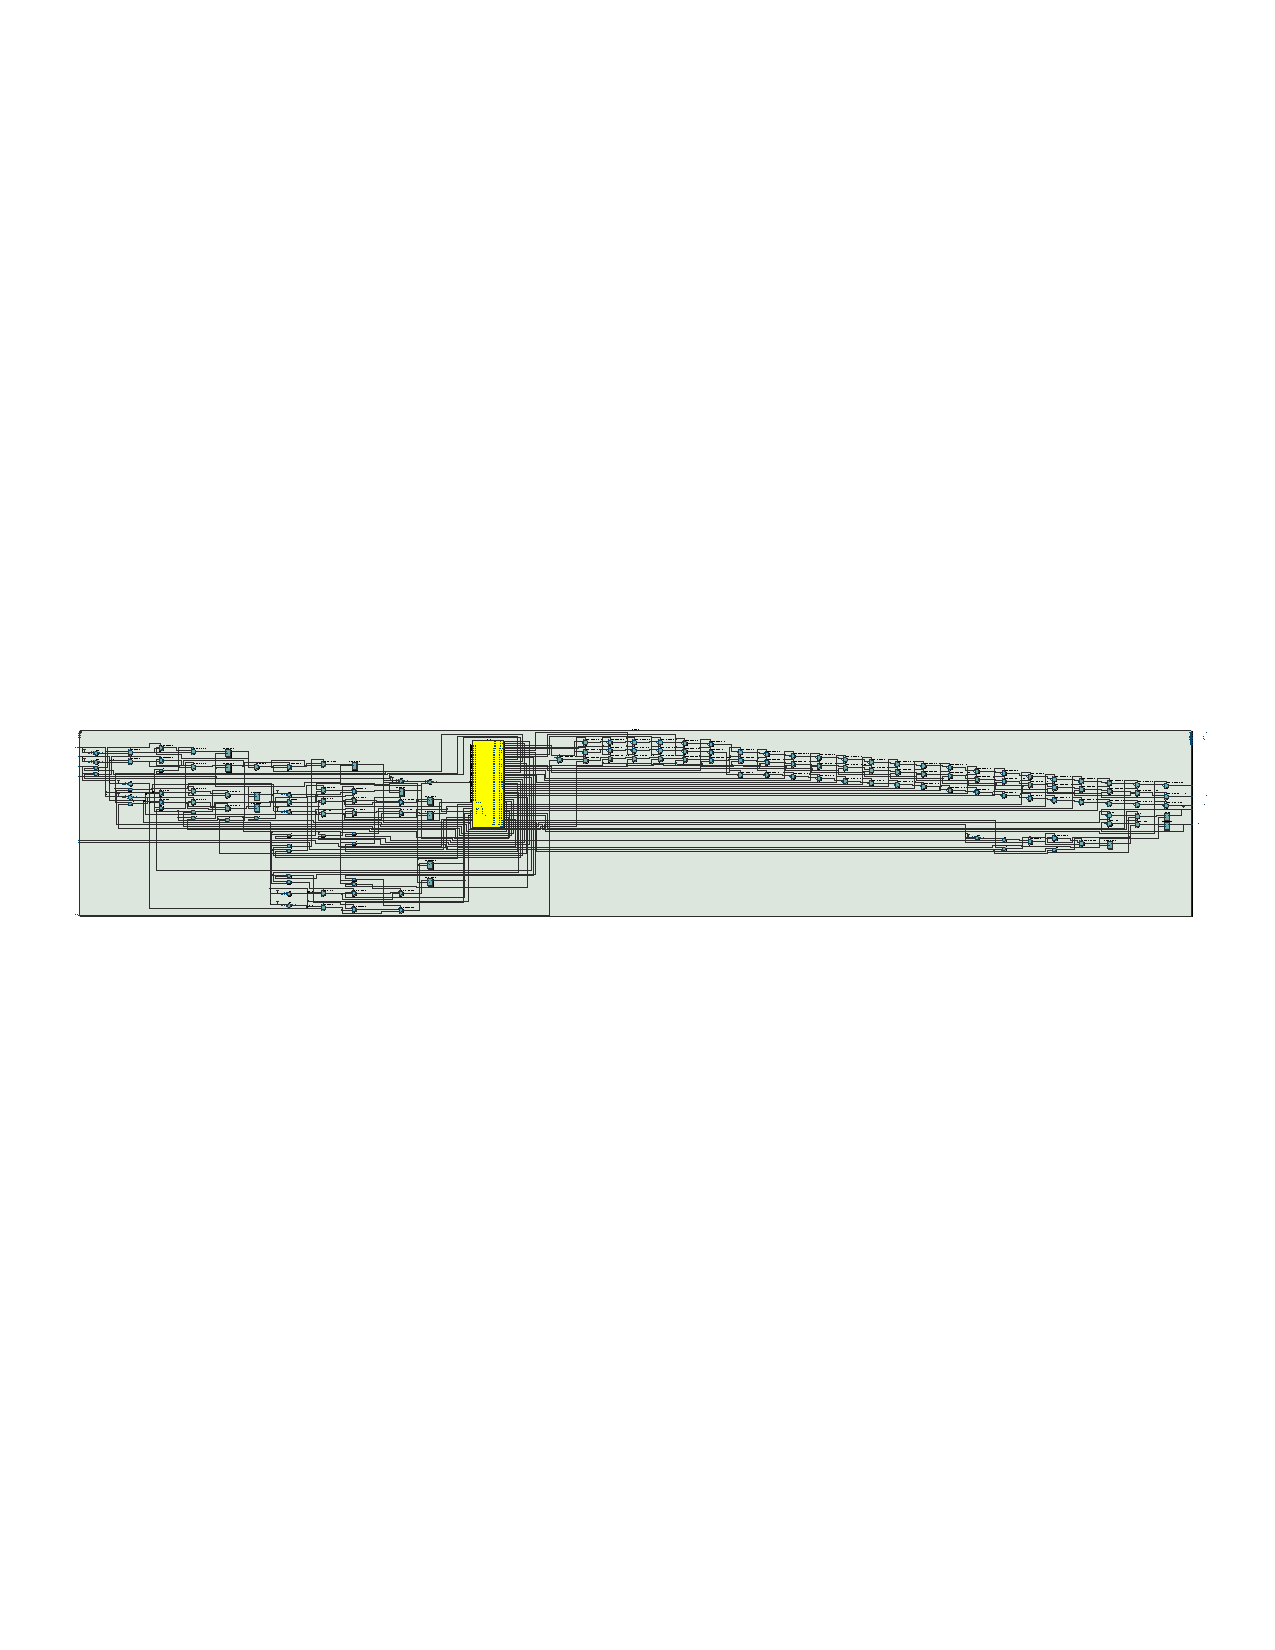
\includegraphics[trim=0.5cm 12cm 0.5cm 10cm, width=\textwidth]{../figs/LegUpOutputMain.pdf}
\caption{\label{fig:legupoumain}Main module of HLS-generated Verilog from LegUp synthesized in Quartus}
\end{figure}

\section{\label{sec:encprob}Encountered problems}
Throughout the work with LegUp, multiple problems that limits its usefulness towards \gls{asic}-applications has been encountered. The following section will describe some of the problems and their implication for the synthesis results described in section \ref{sec:synthres}, as well as for the continuation of the project.
\subsection{\label{subsec:memctrl}Memory controller}
In order to communicate between different modules instantiated in the top-module of the output Verilog from LegUp, a memory controller is declared and instantiated. All variables detected as global by LegUp, i.e. variables used by multiple modules or declared as a pointer and the points-to analysis fails to determine the exact array for the pointer at compile-time, is stored in a \gls{ram} module inside this memory controller. This approach is well intended for the hybrid flow supported by LegUp, where a soft-processor works in cooperation with one or more functions implemented as hardware accelerators in an \gls{fpga}, meaning that data needs to be transferred between the software and hardware portion of the system. For an \gls{asic}, pure-\gls{hw} implementation however, this approach creates a lot of extra overhead and basically does not provide any additional functionality to the circuitry. In the pure-\gls{hw} flow in LegUp, all the functionality described under the main-function in the input C-code will be translated into a single \gls{fsm}. The main function is further the only module instantiated in the top-module of the produced Verilog, besides the memory controller. The use of the memory controller is in itself not an issue as LegUp handles all memory access automatically, but this will come at the expense of both decreased speed and increased area usage. It will also cause some problems related to input and output, as described in subsection \ref{subsec:inoutprobs}.
\subsection{\label{subsec:inoutprobs}Inputs and outputs}
When designing a hardware module, its task can vary almost infinitely. However, most modules take some data input together with some control signals, does something with the data and outputs some kind of response. This makes input and outputs, and the ability to configure them properly, extremely important in most module design. In the documentation of LegUp \cite{leguparch}, the developers claim that each function declared in C is translated into a corresponding module in Verilog. However, \gls{hls}-output shows that in the pure-\gls{hw} flow, the only generated module is the one containing the main-function, as describe in subsection \ref{subsec:memctrl}. As LegUp uses a standard C compiler front-end for \gls{llvm} to compile the C-code into \gls{llvm}-\gls{ir}, we need to follow the \gls{ansi}-C specification \cite{isoc} when writing our C-code. In a standard programming case, the \textit{main}-function has a special purpose, specifically, the run-time environment calls this function to start execution of the program. The return value of the main function is defined to be an int, who's purpose is to return program execution status to the invoker process. The main function is also defined to handle arguments input from command-line, through the input arguments \textit{int argc} and \textit{char *argv[]}, where \textit{argc} is the number of command-line arguments, and \textit{*argv} is an array of pointers to the given arguments. The implications of this is that if we want inputs and outputs to or from the module we design in out C-code, we are limited to the arguments allowed through the defined main-function in the \gls{ansi}-C specifications. Further, this problem increases when we realize that any inputs or outputs except one int for each has to be a pointer, which entails it has to go through the above described memory controller. This causes a lot of overhead, as most input- and output-data has to be written to and read from memory, creating the need for a dedicated custom module for handling I/O. A final issue related to input signals is that the given arguments to the main function in C are not propagated from the generated main module to the top module to make them inputs to the circuit. This means that the designer has to manually alter the generated Verilog to make the the arguments input signals, making it more difficult to create the desired automated framework.
\subsection{Bus widths}
When designing digital hardware circuits, you often want (and in some cases need) to use bit-vectors of a given size. \gls{ansi}-C does not have built-in support for data-types of other sizes than 8, 16, 32 and 64 bits, this cause problems when doing \gls{hls}. LegUp does however have a class, \textit{MinimizeBitwidth.cpp}, which calculate the minimum needed bits in a signal and limits the width to this size, but this does only work for internal signals, where all values assigned to the variable is known at compile-time. If the signal shall be an input or output, the maximum value of the signal is not known, and it can therefore not be limited. Having too wide signals will increase the occupied area as all components must support the extra bits. A simple example is shown in figure \ref{fig:andgate34}, where we can easily see that the addition of one extra bit to the input signal adds one extra 2-input AND gate to the circuit.
\begin{figure}[hbpt]
\centering
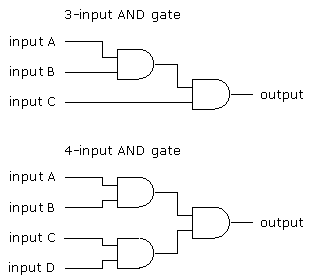
\includegraphics[width=0.6\textwidth]{../figs/AndGate34Bit.png}
\caption{\label{fig:andgate34}3-bit input versus 4-bit input AND-gate}
\end{figure}
Technically this is a limitation inherited from the lack of logical data-types in C, but this problem needs to be addressed if LegUp shall be used as an architectural exploration framework.
\subsection{\label{subsec:parameterprobs}Parameters}
The lack of support for transferring parameters from the C code into the generated Verilog makes it harder to instantiate modules based on widths or depths of different parameters. Often this is desirable in order to reuse the modules for a variety of given parameter values.
\section{\label{sec:synthres}Synthesis results}
Due to the above mentioned problems, some manual alteration of the generated Verilog had to be made in order for the results from LegUp to be comparable to the results from the native Verilog.

\section{Tool-flow and script}
Due to that the \gls{hls}-tool, LegUp, is located on a VirtualBox image while the synthesis and power-estimation tools are located on Nordic's servers, it is not possible to make a single workflow.